
\section{Experimental Methodology}
\label{s:methodology}

Our primary research goal is to evaluate the client-side content-based anti-phishing mechanism and its role in the appearance of warnings shown to the user, including occurrence and timeliness of blacklisting phishing sites within Google Chrome browsers.

On a technical level, in addition to blacklist, major browsers conduct client-side ML-based anti-phishing to evaluate the site to determine if it looks malicious site according to the site features. Based on the classifier threshold, browsers send malicious sites, the client-side classifier results and the website's features to the server to evaluate whether the website is a phishing website~\cite{google-online-security-blog-2019}.

Prior studies of browser-based anti-phishing have focused on the blacklist~\cite{oest2019phishfarm,han2016phisheye,sheng2009empirical}, and the few pieces of research have done in the evasion client-side classifier model. However, these works did not consider users' security in the browsers' content-based anti-phishing system. They also did not evaluate the content-based anti-phishing on blacklisting ratio considering cloaking as a popular evasion method. We perform a comprehensive experiment to satisfy these shortcomings. Figure \ref{ frame work} demonstrates the whole framework we deployed in this paper.
\begin{figure*}[h]
  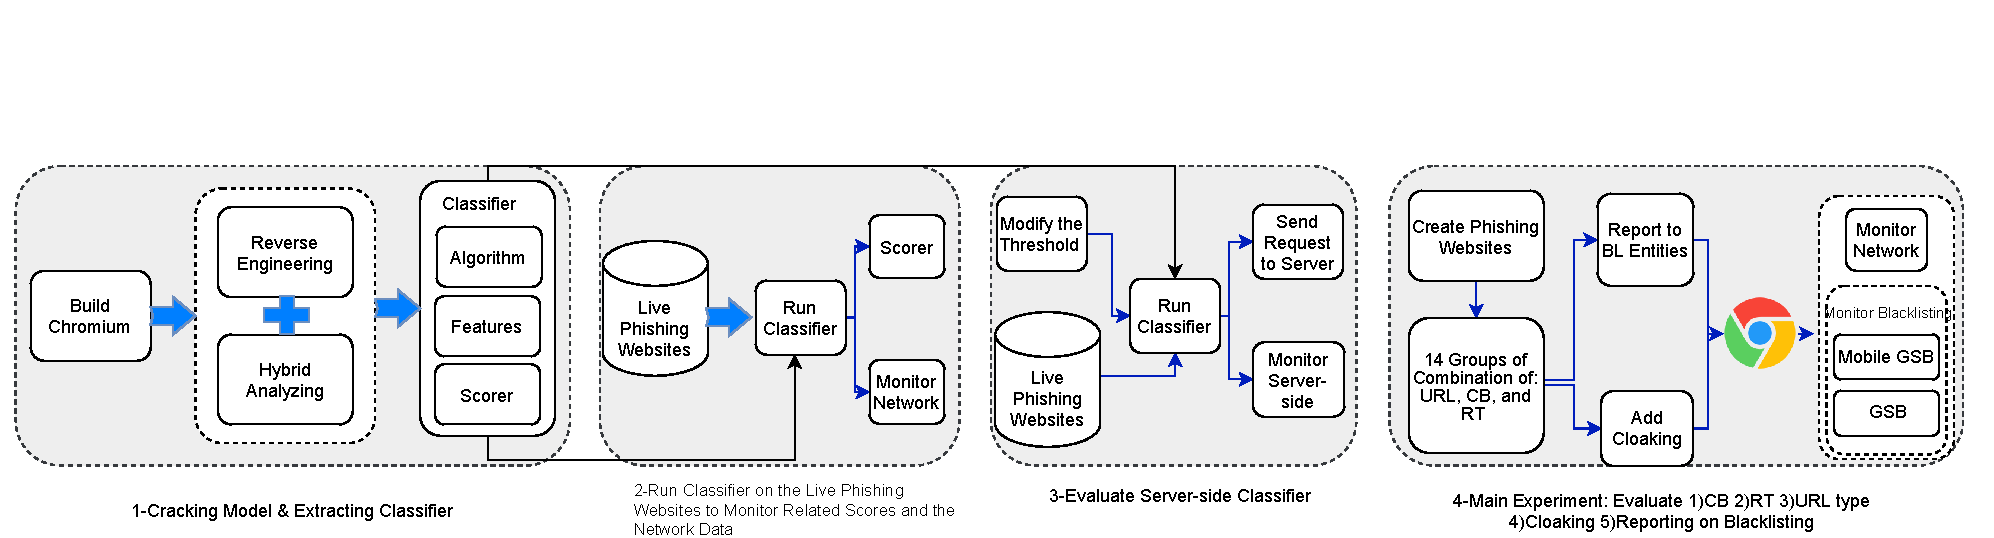
\includegraphics[width=\textwidth,height=6cm]{Untitled Diagram (3).pdf}
  \caption{ Client-side Content-based Anti-phishing Analyzing}
  \label{ frame work}
\end{figure*}

\subsection{Overview}
We dig into the content-based anti-phishing classifier, the machine learning model, the model's changes, real-time anti-phishing, password protection component ~\cite{google-online-security-blog-2019}, all the anti-phishing tools' effect on the blacklisting speed and coverage, and users' privacy in this system.
Our experiment are divided to two main sections:
(1) Classifier experiment includes analysis of Classifier algorithm and scoring results, and evaluating new client-side machine learning model compared to the old model. (2) Blacklist experiment  consists of assessing client-side anti-phishing mechanisms' effects on blacklisting, and analyzing user privacy in the client-side anti-phishing ecosystem .
% \begin{enumerate}
%     \item Classifier experiment: 
%     \begin{enumerate}
%         \item Evaluating Classifier algorithm and scoring results
%         \item Evaluating new client-side machine learning model compared to the old model
%     \end{enumerate}
%     \item Blacklist Experiment:
%     \begin{enumerate}
%         \item Client-side anti-phishing mechanisms' effects on blacklisting
%         \item Analyzing user privacy in the client-side anti-phishing ecosystem
%     \end{enumerate}
% \end{enumerate}
\subsubsection{Classifier experiment}
\textbf{To evaluate classifier algorithm and scoring results:}
In this experiment we extract the whole client-side anti-phishing complex, including classifier's algorithm, features and the phishy-ness score calculating formula. For this part of the experiment, we repeated steps 1-3 from experiment 2.
We have performed this analysis on 100 live phishing sites to extract complete knowledge about the client-side content-based anti-phishing ecosystem. 

\textbf{Evaluating new client-side machine learning model compared to the old mode}:
In September 2020, we realized a noticeable change in the scorer results in the middle of our study. This change appears when we build the chromium source code on a new computer to run a new classifier evaluation experiment.
Chromium is the open-source project behind the google chrome browser. Although Google also adds a number of proprietary features to Chrome, google safe browsing is the same in both chrome and chromium browsers~\cite{the-chromium-projects}. Therefore, we study the GSB source in chromium to analyze the client-side classifier, since it is an open-source project. We deployed the chrome browser in the real-world experiment to evaluate the blacklisting performance. Our study released the main shortcoming of safe browsing during chromium source code analysis. These findings affect other Chromium-based browsers like  Edge version 84.
Deploying reverse engineering on the new source code, we found the source of this mutation in the scorer results. We realized the client-side anti-phishing model and classifier algorithm have changed. Then we decided to add a new experiment to our work to evaluate the newly released client-side machine learning model and find out the effects of this new change on the whole client-side content-based anti-phishing system. 

We considered two factors in comparison to the results of the classifier on old and new phishing websites:
\begin{enumerate}
    \item Improvement of the client-side machine learning model
    \item The improvement of the phishers knowledge about defeating the client-side classifier( The advancement of the URL and content of the phishing websites to misclassify by the client-side machine learning model)
\end{enumerate}

This experiment is described in the following steps: we repeated steps 1-3 from experiment 2, and We collected phishing websites for earlier years.
% \begin{enumerate}
%     \item We repeated steps 1-3 from experiment 2.
%     \item We collected phishing websites for earlier years.
% \end{enumerate}

To perform an accurate comparison between the new and old models, we consider that the growth in sophistication of recent phishing attacks may weaken the classifier's results with the new model. Therefore, we run two models on old and new phishing websites.
Since phishing websites' lifetime is not long, we could not access old phishing websites using their URLs.For this purpose, we used the KitPhisher tool~\cite{cybercdh} to obtain phish kits for 2016 and redeploy the phishing websites for 2016.
Phish kits are a unified set of tools that phishers use to deploy a phishing site on a server~\cite{mccalley2011analysis}. The study conducted in 2018~\cite{oest2018inside} showed that the phishing kits started to provide different types of cloaking to make the phishing attacks more sophisticated. To provide phish kits without these techniques, we used phish kits of two years earlier than the time that this study has implemented.

\subsubsection{Blacklisting experiment}
In this section, we discuss three metrics that we consider to evaluate blacklists. We also explain the experiment structure as well as the specific blacklist that we use in our study. 

The blacklist performance metrics are described in table~\ref{tab:Blacklisting metrics}. We consider blacklist's ability to discover new suspected URLs
(\textit{Discovery})as one performance parameter, and blacklist's ability to blacklisting discovered URLs (\textit{Detection})  as another performance metric. To evaluate detection parameter we use two sub-metrics: \textit{Coverage} and \textit{Speed}~\cite{oest2020phishtime} that also are briefly explained in table~\ref{tab:Blacklisting metrics}. 
We focus our study on GSB due to its large potential impact. However, our methodology and framework could be applied to evaluate other blacklist providers such as \textit{Microsoft SmartScreen}, \textit{Opera’s fraud and malware protection}, and other alternatives.

To perform an effective evaluation of client-side content-based anti-phishing, we deploy a large batch of phishing websites, using different browser settings combined with evasion methods and reporting some of these groups directly to blacklists, then monitor all the websites to see blacklisting coverage and timeliness. Meanwhile, we monitor network traffic to analyze the user's privacy in this ecosystem and understand the browser's interactions at the GSB backend.


\begin{table}
\centering
\scalebox{0.93}{
\begin{tabular}{lll} 
\hline
\toprule
\multicolumn{2}{l}{\begin{tabular}[c]{@{}l@{}}BL Performance\\ Metrics \end{tabular}} & Description                                                                                                                     \\ 
\hline
\multicolumn{2}{l}{Discovery}                                                         & \begin{tabular}[c]{@{}l@{}}\small{Blacklist’s ability to identify}\\\small{new suspected URLs}\end{tabular}                                      \\
\hline
\multirow{2}{*}{Detection} & Coverage                                                 & \begin{tabular}[c]{@{}l@{}}\small{The proportion of the discovered}\\ \small{URLs that are correctly blacklisted\\ at any point} \end{tabular}  \\ 
\cline{2-3}
                           & Speed                                                    & \begin{tabular}[c]{@{}l@{}}\small{The time delay between} \\\small{discovery and blacklisting} \end{tabular}                                    \\

\bottomrule
\end{tabular}}
\caption{Blacklisting evaluation metrics~\cite{oest2020phishtime}}
\label{tab:Blacklisting metrics}
\end{table}

On the other hand, to empirically evaluate the server-side anti-phishing classifier's performance, we use a large group of live phishing websites from PhishTank and send them to the server-side classifier with and monitor the server responses.
At a high level,We deploy our phishing websites on a large scale. 

We consider 14 batches to cover the different combinations of browser settings and implementation of cloaking, and reporting to the blacklist entities in different ways. We assign 35 sites for each group. In May 2020, we created a total of 490 new phishing websites to evaluate content-based anti-phishing in terms of different browser defense layers and cloaking.We performed direct observations of blacklisting across these different batches for the Google Safe browsing experiment. 

For five batches, once the sites are live, we report their URLs to the anti-phishing entities being tested. We then monitor the entity's response and record the crawling logs, including the time of entities' and blacklist API's visit and blacklisting. Meanwhile, we collect network data for each website.

In our experiments, we used the phishing sites that all spoofed the Paypal.com login page with permission from PayPal, Inc. All the phishing sites that we used each used new, unique, and previously-unseen .com domain names. We measure the time between our report and browser blacklisting for each site and for doing the experiment more reliably; we did not use any domain more than once.  
This experiment steps are described below:  

\begin{enumerate}
    \item Selecting a specific group of anti-phishing entities to test
    \item Configuring Chrome browser to deploying experiment on, Deploying three Virtual Machines (for three different settings of chrome browser) for running the experiment and implement experiment infrastructure on all of them, and Deploying a network traffic capture tool on each Virtual Machine
    \item Creating 490 new, unique, and previously-unseen PayPal phishing sites with desired cloaking techniques
    \item Deploy a batch of phishing websites for different browser settings, reporting, and cloaking
    \item Reporting 5 groups of the websites to the entities
    
\end{enumerate}

We run the experiment for seven days. When experiment is finished we measure the blacklisting time( the time between reporting and blacklisting) from the log file. We also have the blacklisting result for all the websites.


